\subsection{Experiment \#1}\label{subsec:exp1}
% Experiment structure
%
% Intro:
%   - background
%   - goal / experiment intention / why
%   - data
%   - evaluation
%   - reference to result table
%
% Procedure (by data if more than one):
%   - pre-processing
%   - feature extraction
%   - mapping
%   - feature representation
%   - classifier
%
% Remarks (if any)
%
% Result highlights:
%   - (only a description)

%% Experiment intro
This experiment intends to find the optimal number of words and its effect on the different configurations (i.e., pre-processing and feature representation), on the contrary to~\cite{Lemaintre2015miccaiOCT}, where the codebook size was arbitrarily set to $k = 32$.

%(pre-processing which consists of denoising, flattening, and aligning along different mapping).
%In order to determine the optimal size of the codebook when using \bow, this experiment evaluates several codebook sizes on SERI dataset.

%% Experiment procedure
Several pre-processing strategies are used: (i) \ac{nlm}, (ii) a combination of \ac{nlm} and flattening (\ac{nlm}+\f), and (iii) a combination of \ac{nlm}, flattening, and aligning (\ac{nlm}+\fal).
\lbp and \lbptop descriptors are detected using the default configuration.
Volumes are represented using \ac{bow}, where the codebook size ranging for $k\in \{10, 20, 30, \cdots, 100, 200, \cdots, 500,$ $1000\}$.
Finally, the volumes are classified using \lr.
The choice of this linear classifier avoids that the results get boosted by the classifier.
In this manner, any improvement would be linked to the pre-processing and the size of the codebook.
%
\begin{landscape}

  \begin{table}
\caption{Experiment \#1 - Optimum number of words for each configuration as a result of \ac{lr} Classification, for high-level feature extraction of \emph{global} and \emph{local}-\ac{lbp}, and \emph{local}-\ac{lbptop} features with different pre-processing. The pre-processing includes: \ac{nf}, \ac{f}, and \ac{fal}.
The achieved performances are indicated in terms of  \acs{acc}, \acs{f1}, \acs{se}, and \acs{sp}}
\centering

\footnotesize{
\resizebox{1\linewidth}{!}{
\begin{tabular}{ll  ccccr	c	ccccr	c ccccr}
\toprule
Features & Pre-processing &    \multicolumn{5}{c}{$\{8,1\}$}  & & \multicolumn{5}{c}{$\{16,2\}$} & & \multicolumn{5}{c}{$\{24,3\}$} \\
  \cmidrule(l){3-7}  \cmidrule(l){9-13}  \cmidrule(l){15-19}
   & &  	\ac{acc}\% & \ac{f1}\% & \ac{se}\% & \ac{sp}\%  & W\# &  & \ac{acc}\% & \ac{f1}\% & \ac{se}\% & \ac{sp}\%  & W\# &  &\ac{acc}\% & \ac{f1}\% & \ac{se}\% & \ac{sp}\%  & W\# \\
\midrule
\\[-2ex]
  	\emph{global}-\ac{lbp}		\\
 	& \acs{nf} & 81.2 &  78.5 & 68.7 &  93.7 & 500 & & 62.5 & 58.0 & 56.2 & 62.5 & 80  & & 62.5  & 62.5 & 62.5 & 62.5 & 80  \\
	& \acs{f}  & 71.9 &  71.0 & 68.7 &  75.0 & 400 & & 68.7 & 66.7 & 62.5 & 75.0 & 300 & & 68.7  & 66.7 & 62.5  & 75.0 & 300	 \\
	& \acs{fal}& 71.9 &  71.0 & 68.7 &  75.0 & 500 & & 71.9 & 71.0 & 68.7 & 75.0 & 200 & & 75.0  & 68.7 & 68.7  & 68.7 & 500	 \\
	%& \acs{fac}& 75.0 & 73.3 & 68.7 &  81.2 & 500 & & 78.1 & 75.8 & 68.7 & 87.5 & 500 & & 68.7  & 68.7 & 68.7  & 68.7 & 90	 \\
	\\
\hdashline \noalign{\vskip 3pt}
\\[-2ex]
 	\emph{local}-\ac{lbp}		\\
 	& \acs{nf}  &\cellcolor[gray]{0.6}75.0  &\cellcolor[gray]{0.6} 75.0 &\cellcolor[gray]{0.6} 75.0  &\cellcolor[gray]{0.6} 75.0 &\cellcolor[gray]{0.6} 70 & & 65.6 & 64.5 & 62.5 & 68.7 & 90 & &  62.5 & 60.0 & 56.2  & 68.7  & 30  \\
	& \acs{f}   & 75.0  & 73.3 & 68.7  & 81.2 & 30 & & 71.8 & 61.0 & 68.7 & 75.0 & 70 & &  62.5 & 62.5 & 62.5  & 62.5  & 100	 \\
	& \acs{fal} & 75.0  & 69.0 & 62.5  & 81.2 & 40 & & 71.9 & 71.0 & 68.7 & 75.0 & 200 & &  68.7 & 66.7 & 68.7 & 62.5 & 10	 \\
	%& \acs{fac}& 68.7 & 68.7 & 68.7 & 68.7 & 300 & & 65.6 & 64.5 & 62.5 & 68.7 & 100 & & 65.6  & 64.5 & 62.5  & 68.7 & 100	 \\
	\\
\hdashline \noalign{\vskip 3pt}
\\[-2ex]
 	\emph{local}-\ac{lbptop}		\\
 	& \acs{nf}	& 68.7 & 68.7 & 68.7 & 68.7 & 400 & & \cellcolor[gray]{0.6}75.0  & \cellcolor[gray]{0.6}75.0   &\cellcolor[gray]{0.6}75.0   &\cellcolor[gray]{0.6}75.0  &\cellcolor[gray]{0.6}500 & & 71.9 & 71.0 & 68.7 & 75.0 & 60	 \\
	& \acs{f}	& 68.7 & 68.7 & 68.7 & 68.7 & 300 & & 68.7  & 66.7   & 62.5   & 75.0  & 50  & & 75.0 & 76.5 & 81.2 & 68.7 & 80	 \\
	& \acs{fal}	& 75.0 & 73.3 & 68.7 & 81.2 & 100 & & 75.0  & 73.3   & 68.7   & 81.2  & 90  & & 75.0 & 69.0 & 62.5 & 81.2 & 70	 \\
	%& \acs{fac}	& 71.9 & 69.0 & 62.5 & 81.2 & 400 & & 75.0  & 73.3   & 68.7   & 81.2  & 100 & & 75.0 & 73.3 & 68.7 & 81.2 & 60	 \\
	\\

\bottomrule
\end{tabular}}}
\label{tab:table2}
\end{table}
\end{landscape}



The usual build of the codebook consists of clustering the samples in the feature space using $k$-means (see Sect.\,\ref{subsec:fearep}).
However, this operation is rather computationally expensive and the convergence of the $k$-means algorithm for all codebook sizes is not granted.
Nonetheless, Nowak\,\textit{et al.}~\cite{nowak2006sampling} pointed out that randomly generated codebooks can be used at the expenses of accuracy.
Thus, the codebook are randomly generated since the final aim is to asses the influence of the codebook size and not the performance of the framework.
For this experiment, the codebook building is carried out using random initialization using $k$-means++ algorithm~\cite{arthur2007k}, which is usually used as a $k$-means initialization algorithm.

For this experiment, \ac{se} and \ac{sp} are complemented with \ac{acc} and \ac{f1} score (see Eq.\,\eqref{eq:accf1}).
\ac{acc} offers an overall sense of the classifier performance, and \ac{f1} illustrates the trade off between \ac{se} and precision.
Precision or positive predictive value is a measure of algorithm exactness and is defined as a ratio of \ac{tp} over the total predicted positive samples.
\begin{align}
\ac{acc} = \frac{TP+TN}{TP+TN+FP+FN} \qquad \ac{f1} = \frac{2TP}{2TP +FP+FN}
\label{eq:accf1}
\end{align}
Appendix~\ref{app:1}~-~Table~\ref{tab:table2} shows the results obtained for the optimal dictionary size while the complete set of all \ac{acc} and \ac{f1} graphics can be found at~\cite{Lemaitre2015}.
According to the obtained results, it is observed that optimum number of words is smaller for \emph{local}-\ac{lbp} features in comparison to \emph{local}-\ac{lbptop} and \emph{global}-\ac{lbp}, respectively.
Using \ac{lr} classifier, the best performances were achieved using \emph{local}-\ac{lbp} with 70 words (\ac{se} and \ac{sp} of 75.0\%) and \emph{local}-\ac{lbptop} with 500 words (\ac{se} and \ac{sp} of 75.0\% as well).
These results are highlighted in Appendix~\ref{app:1}~-~Table~\ref{tab:table2}.





%In order to illustrate the impact of the dictionary size, Fig.\,\ref{fig:RBOW} illustrates the \ac{acc} and \ac{f1} graph for a particular case.
%In this figure, the classification performance of \emph{local}-\ac{lbp} features extracted from the \nlm+\f configuration is illustrated. 
%\begin{figure}
%\centering
%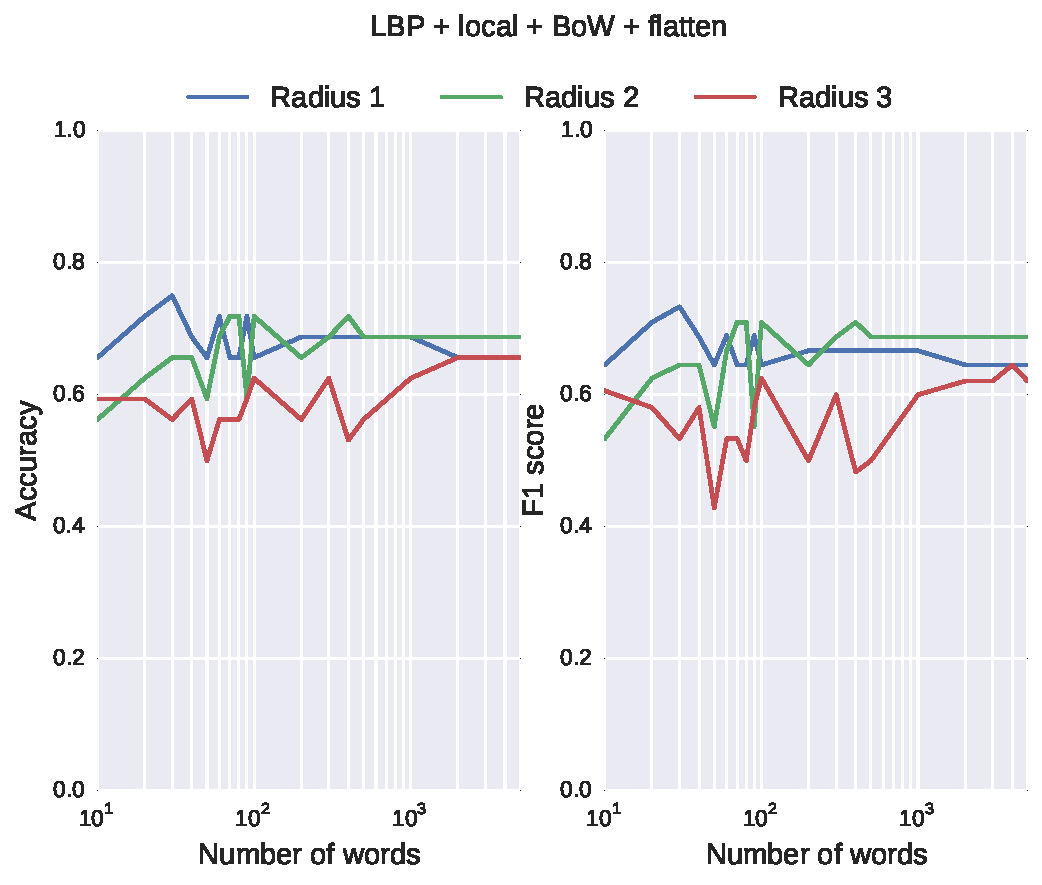
\includegraphics[width=0.85\textwidth]{figure2}
%\caption{The performance of \ac{lr} with NLM+\ac{f} pre-processing for different $P$ and $R$.}
%\label{fig:RBOW}
%\end{figure}
%%% Experiment Result description
%The obtained results show that commonly less number of words is required when higher number of sampling points and radius ($\{P,R\} = \{24,3\}$) are used.
%The required number of words decreases for \emph{local}-\ac{lbp} in comparison with \emph{global}-\ac{lbp}.
%Although it was expected that the use of different pre-processing steps affect the optimal number of words, this influence is not substantial nor consistent over all the obtained results.


